\documentclass{article}
\usepackage{fancyhdr}
\usepackage{ctex}
\usepackage{listings}
\usepackage{graphicx}
\usepackage[a4paper, body={18cm,22cm}]{geometry}
\usepackage{amsmath,amssymb,amstext,wasysym,enumerate,graphicx}
\usepackage{float,abstract,booktabs,indentfirst,amsmath}
\usepackage{array}
\usepackage{booktabs}
\usepackage{multirow}
\usepackage{url}
\usepackage{diagbox}
\renewcommand\arraystretch{1.4}
\usepackage{indentfirst}
\setlength{\parindent}{2em}
\usepackage{enumerate}
\setmonofont{MesloLGS NF}
\usepackage{listings}
\usepackage{xcolor}
\lstset{
    language = C,
    xleftmargin = 3em,xrightmargin = 3em, aboveskip = 1em,
	backgroundcolor = \color{white}, % 背景色
	basicstyle = \normalsize\ttfamily, % 基本样式 + 小号字体
	rulesepcolor= \color{gray}, % 代码块边框颜色
	breaklines = true, % 代码过长则换行
	numbers = left, % 行号在左侧显示
	numberstyle = \small, % 行号字体
    numbersep = -14pt, 
	keywordstyle = \color{blue!50!red!100}, % 关键字颜色
	commentstyle =\color{red!50!green!50!blue!60}, % 注释颜色
	stringstyle = \color{red}, % 字符串颜色
	frame = shadowbox, % 用(带影子效果)方框框住代码块
	showspaces = false, % 不显示空格
	columns = fixed, % 字间距固定
} 
%--------------------页眉--------------------%
\pagestyle{fancy}
\fancyhead[L]{}
\fancyhead[R]{}
\fancyhead[C]{华东师范大学软件工程学院实验报告}
\fancyfoot[C]{-\thepage-}
\renewcommand{\headrulewidth}{1.5pt}
%--------------------标题--------------------%
\begin{document}
\begin{center}
    \LARGE{{\textbf{\heiti 华东师范大学软件工程学院实验报告}}}
    \begin{table}[H]
        \centering
        \begin{tabular}{p{2cm}p{4cm}<{\centering}p{1cm}p{2cm}p{4cm}<{\centering}}
            姓\qquad 名: & 李鹏达 & \quad & 学\qquad 号: & 10225101460       \\ \cline{2-2} \cline{5-5}
            实验编号:    & Lab 01 & \quad & 实验名称:    & Manipulating bits
            \\ \cline{2-2} \cline{5-5}
        \end{tabular}
    \end{table}
\end{center}
\rule{\textwidth}{1pt}
%--------------------正文--------------------%
\section{实验目的}
\large
\begin{enumerate}[1)]
    \item 熟悉整数和浮点数的位级表示
    \item 练习C中位运算的使用
\end{enumerate}
\normalsize
\section{实验内容与实验步骤}
\subsection{实验内容}
\large
编写完善bits.c中关于整数和浮点数位级表示的15个函数,并进行评测。
\paragraph{1) bitAnd}
要求仅使用$\sim$和 | 完成 \& 操作。

考虑到 x \& y = $\sim$$\sim$(x \& y) = $\sim$($\sim$x | $\sim$y),代码如下:
    \begin{lstlisting}[language=C]
    int bitAnd(int x, int y) {
        return ~(~x | ~y);
    }
\end{lstlisting}
    \paragraph{2) getByte}
    获取x第n个字节的内容

    将x右移$n\times 8$位(一字节)后与0xff相与,代码如下:
    \begin{lstlisting}[language=C]
    int getByte(int x, int n) {
        return (x >> (n << 3)) & 0xff;
    }
\end{lstlisting}
    \paragraph{3) logicalShift}完成逻辑右移功能

    先进行算数右移,然后再与一个前n位全为零而其他位全为1的数相与,从而对先n位进行清零,代码如下:
    \begin{lstlisting}[language=C]
    int logicalShift(int x, int n) {
        return (x >> n) & ~(1 << 31 >> n << 1);
    }
\end{lstlisting}
    \paragraph{4) bitCount} 统计一个数的二进制表示中1的个数

    首先定义5个掩码(mask1到mask5)用于按位操作。这些掩码的作用是将整数x中的每个不同位按组分组,并将相邻的位相加,以便计算每组中包含的1的数量。然后将掩码mask1-5应用于x,以按2位、4位、8位、16位和32位分组计算1的数量。最后,将所有组中1的数量相加,得到结果,代码如下:
    \begin{lstlisting}[language=C]
    int bitCount(int x) {
        int mask1 = 0x55 | 0x55 << 8;
        int mask2 = 0x33 | 0x33 << 8;
        int mask3 = 0x0f | 0x0f << 8;
        int mask4 = 0xff | 0xff << 16;         // 0x00ff00ff
        int mask5 = 0xff | 0xff << 8;          // 0x0000ffff
        mask1 = mask1 | mask1 << 16;           // 0x55555555
        mask2 = mask2 | mask2 << 16;           // 0x33333333
        mask3 = mask3 | mask3 << 16;           // 0x0f0f0f0f
        x = (x & mask1) + ((x >> 1) & mask1);  // add count of 1 every 2 bits
        x = (x & mask2) + ((x >> 2) & mask2);  // every 4 bits
        x = (x & mask3) + ((x >> 4) & mask3);  // every 8 bits
        x = (x & mask4) + ((x >> 8) & mask4);  // every 16 bits
        x = (x & mask5) + ((x >> 16) & mask5); // every 32 bits
        return x;
    }
\end{lstlisting}
    \paragraph{5) bang} 在不使用!的情况下得到!x

    首先将x与其相反数按位或,在x是0的情况下得到0,其他情况下得到最高位为1的二进制数。右移31位并按位取反后,0得到全1而其他情况得到全0,与1相与得到答案。代码如下:
    \begin{lstlisting}[language=C]
    int bang(int x) {
        return ~((x | (~x + 1)) >> 31) & 1; 
        // the highest bit of x | (~x + 1) is 0 only if x = 0
    }
\end{lstlisting}
    \paragraph{6) tmin} 得到int类型整数的最小值

    即0x80000000,代码如下:
    \begin{lstlisting}[language=C]
    int tmin(void) {
        return 1 << 31;
    }
\end{lstlisting}
    \paragraph{7) fitsBits} 判断x是否能被表示成n位二进制补码

    如果x左移$32-n$位再右移$32-n$后结果不变,则x可以被表示成n位二进制补码,代码如下:
    \begin{lstlisting}[language=C]
    int fitsBits(int x, int n) {
        int c = 33 + ~n; // 32 - n
        return !(((x << c) >> c) ^ x); 
        // x ^ y equals 0 only if x == y 
    }
\end{lstlisting}
    \paragraph{8) divpwr2} 计算$\frac{x}{2^n}$, 向0舍入。

    考虑通过右移代替除法,但其对数字的直接截断在$x<0$时不满足向0舍入的要求。考虑设置一个偏移量bias,当$x<0$时,将其设置为$2^n-1$,以对x进行修正,完成向0舍入。代码如下:
    \begin{lstlisting}[language=C]
    int divpwr2(int x, int n) {
        int bias = (x >> 31) & ((1 << n) + ~0); 
        // equals 0 when x >= 0 and 2 ^ n - 1 when x < 0
        return (x + bias) >> n;
    }
\end{lstlisting}
    \paragraph{9) negate} 得到$-x$

    即$\sim x + 1$,代码如下:
    \begin{lstlisting}[language=C]
    int negate(int x) {
        return ~x + 1;
    }
\end{lstlisting}
    \paragraph{10) isPositive} 判断$x>0$是否成立

    考虑将x右移31位以提取符号位,但要注意特判$x=0$,此时应返回0,代码如下:
    \begin{lstlisting}[language=C]
    int isPositive(int x) {
        return (!(x >> 31)) & !!x;
    }
\end{lstlisting}
    \paragraph{11) isLessOrEqual} 判断$x \le y$是否成立

    考虑通过判断$y-x\ge 0$是否成立来进行判断。但在$x<0$且$y>0$,或$x>0$且$y<0$时,可能发生溢出,不过在前一种情况下,$x \le y$必然成立,后一种情况下必然不成立,直接特判即可。代码如下:
    \begin{lstlisting}[language=C]
    int isLessOrEqual(int x, int y) {
        int ispositivex = !(x >> 31);             // x >= 0
        int ispositivey = !(y >> 31);             // y >= 0
        return (!ispositivex | ispositivey)       // !(x > 0 && y < 0)
                & (((!ispositivex) & ispositivey) // x < 0 && y > 0
                | !(((y + ~x + 1) >> 31) & 1));   // y - x >= 0
    }
\end{lstlisting}
    \paragraph{12) ilog2} 计算$\log_2 x$

    $\log_2 x$的值即为x的二进制表示中最高位的位置。可以采用类似分治的思路,从16位到8位,4位,2位,1位,逐步确定x的最高位的位置,代码如下:
\begin{lstlisting}[language=C]
    int ilog2(int x) {
        int ans = ((!!(x >> 16)) << 4);
        ans = ans | ((!!(x >> (ans + 8))) << 3);
        ans = ans | ((!!(x >> (ans + 4))) << 2);
        ans = ans | ((!!(x >> (ans + 2))) << 1);
        ans = ans | (!!(x >> (ans + 1)));
        return ans;
    }
\end{lstlisting}  
\paragraph{13) float\_neg} 计算浮点数f的相反数,但当f是NaN时,返回f

将f的最高位取反即可,但要注意特判NaN。代码如下:
\begin{lstlisting}[language=C]
    unsigned float_neg(unsigned uf) {
        if (!(((uf << 1) ^ 0xff000000) >> 24) & !!(uf & 0x007fffff))
          return uf;
        else
          return uf + 0x80000000;
    }
\end{lstlisting}  

\paragraph{14) float\_i2f} 将整数转换为浮点数

可以通过将ux循环右移得到最高位的位置,进而加上偏移量得到阶码值$e$。注意将int类型整数转换为单精度浮点数时,需要舍去最后9位,因此需要注意浮点数表示规则中的向偶数舍入。当最后9位大于0x100时,或最后十位为0x300时,满足要求,将结果加一。在代码中,$e$的初始值被设置为$bias-1$,这是因为在二进制表示中,最后一位的权值是$2^0$。代码如下:
\begin{lstlisting}[language=C]
    unsigned float_i2f(int x) {
        unsigned ux = x < 0 ? -x : x;
        unsigned _ux = ux;
        unsigned e = 127 - 1; // bias - 1
        unsigned ans = 0;
        unsigned frac;
        int shift = 0; // bits to shift left
        int flag;      // round-to-even
        while (ux) {
          e++;
          ux >>= 1;
        }
        if (x == 0) {
          return 0;
        } else if (x < 0) {
          ans |= 0x80000000;
        }
        shift = 159 - e; // 32 - (e - 127)
        frac = _ux << shift;
        flag = (frac & 0x1ff) > 0x100 || (frac & 0x3ff) == 0x300;
        frac = frac >> 9; // 32 - 23
        return (ans | (e << 23) | frac) + flag;
    }
\end{lstlisting}  
\paragraph{15) float\_twice} 计算一个浮点数的两倍,但当f是NaN时,返回f

分情况讨论。当f是规格化的浮点数时,直接将阶码加一,当x是非规格化的浮点数时,直接将尾数乘以2,当f是NaN时,不变。代码如下:
\begin{lstlisting}[language=C]
    unsigned float_twice(unsigned uf) {
        if ((uf & 0x7f800000) == 0) {                      
            // is denormalized
            uf = (uf & 0x007fffff) << 1 | (uf & 0x80000000); 
            // frac *= 2
        } else if ((uf & 0x7f800000) != 0x7f800000) {      
            // is not NaN
            uf += 0x00800000; // exp += 1
        }
        return uf;
    }
\end{lstlisting}  

\normalsize

\subsection{实验步骤}
\large
\begin{enumerate}[1)]
    \item 安装必要的软件和库,如make, gcc-multilib等
    \begin{lstlisting}[language=bash]
    linux> sudo apt install make gcc gcc-multilib
    \end{lstlisting}  
    \item 将datalab-handout在Linux下进行解打包
    \begin{lstlisting}[language=bash]
    linux> tar -xvf datalab-handout
    \end{lstlisting} 
    \item 编辑bits.c,完成其中的15个函数
    \item 编译
    \begin{lstlisting}[language=bash]
    linux> make
    \end{lstlisting} 
    \item 运行driver.pl进行评测
    \begin{lstlisting}[language=bash]
    linux> ./driver.pl
    \end{lstlisting} 
\end{enumerate}
\normalsize
\section{实验过程与分析}
\large
在实验过程中,我遇到了一些困难和问题。

首先便是题目的难度较高。bitCount和ilog2两题在独立思考较长时间后,仍没有较好的思路,在网上查阅资料后,最终才完成这两题。在某些题目的舍入上也遇到了一些问题,讲过多次修改最终才通过测试。

在实验中,我还遇到了一些BUG。在题目fitsBits的评测中,似乎出现了一些问题。起初,我是用的平台为WSL2中的Ubuntu 20.04.6 LTS,内核版本为5.15.90.1-microsoft-standard-WSL2,gcc版本为9.4.0。在评测fitsBits时,我遇到了错误

\begin{lstlisting}
    ERROR: Test fitsBits(-2147483648[0x80000000],32[0x20]) failed...
    ...Gives 1[0x1]. Should be 0[0x0]
\end{lstlisting} 
然而,0x80000000明显时可以用32位补码表示的。
后来,我用相同的代码在Vmware中的Ubuntu 20.04.6 LTS上重新进行了评测,其内核版本为5.0.0-23-generic,gcc版本为7.5.0。在此版本的Linux上,没有遇到这个问题。经过我在网上的搜索和线下的实践,我怀疑此BUG可能与gcc版本有关。

实验最后的评测截图如下:
\begin{figure}[h]
    \centering
    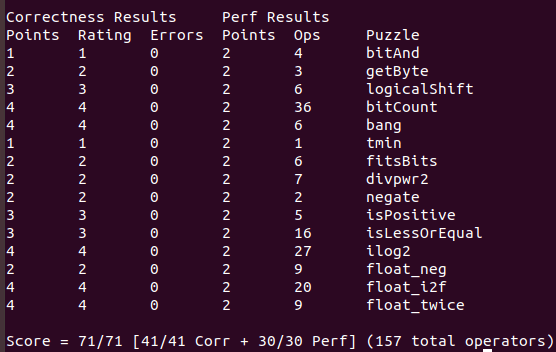
\includegraphics[width=15cm]{lab1.png}
    \caption{评测截图}
\end{figure}

\normalsize
\section{实验结果总结}
\large
通过本次实验,我进一步深入理解了整数和浮点数的位级表示,同时,也学习到了在C语言中进行有关位运算的一些技巧,还了解到了一些Linux上的基本操作。
\normalsize
\section{附录(源代码)}
\large
bits.c的源代码如下(此代码已同时以文件的形式提交):
\begin{lstlisting}[language=C]
    /* 
    * CS:APP Data Lab 
    * 
    * <Please put your name and userid here>
    * 
    * bits.c - Source file with your solutions to the Lab.
    *          This is the file you will hand in to your instructor.
    *
    * WARNING: Do not include the <stdio.h> header; it confuses the dlc
    * compiler. You can still use printf for debugging without including
    * <stdio.h>, although you might get a compiler warning. In general,
    * it's not good practice to ignore compiler warnings, but in this
    * case it's OK.  
    */
   
   #if 0
   /*
    * Instructions to Students:
    *
    * STEP 1: Read the following instructions carefully.
    */
   
   You will provide your solution to the Data Lab by
   editing the collection of functions in this source file.
   
   INTEGER CODING RULES:
    
     Replace the "return" statement in each function with one
     or more lines of C code that implements the function. Your code 
     must conform to the following style:
    
     int Funct(arg1, arg2, ...) {
         /* brief description of how your implementation works */
         int var1 = Expr1;
         ...
         int varM = ExprM;
   
         varJ = ExprJ;
         ...
         varN = ExprN;
         return ExprR;
     }
   
     Each "Expr" is an expression using ONLY the following:
     1. Integer constants 0 through 255 (0xFF), inclusive. You are
         not allowed to use big constants such as 0xffffffff.
     2. Function arguments and local variables (no global variables).
     3. Unary integer operations ! ~
     4. Binary integer operations & ^ | + << >>
       
     Some of the problems restrict the set of allowed operators even further.
     Each "Expr" may consist of multiple operators. You are not restricted to
     one operator per line.
   
     You are expressly forbidden to:
     1. Use any control constructs such as if, do, while, for, switch, etc.
     2. Define or use any macros.
     3. Define any additional functions in this file.
     4. Call any functions.
     5. Use any other operations, such as &&, ||, -, or ?:
     6. Use any form of casting.
     7. Use any data type other than int.  This implies that you
        cannot use arrays, structs, or unions.
   
    
     You may assume that your machine:
     1. Uses 2s complement, 32-bit representations of integers.
     2. Performs right shifts arithmetically.
     3. Has unpredictable behavior when shifting an integer by more
        than the word size.
   
   EXAMPLES OF ACCEPTABLE CODING STYLE:
     /*
      * pow2plus1 - returns 2^x + 1, where 0 <= x <= 31
      */
     int pow2plus1(int x) {
        /* exploit ability of shifts to compute powers of 2 */
        return (1 << x) + 1;
     }
   
     /*
      * pow2plus4 - returns 2^x + 4, where 0 <= x <= 31
      */
     int pow2plus4(int x) {
        /* exploit ability of shifts to compute powers of 2 */
        int result = (1 << x);
        result += 4;
        return result;
     }
   
   FLOATING POINT CODING RULES
   
   For the problems that require you to implent floating-point operations,
   the coding rules are less strict.  You are allowed to use looping and
   conditional control.  You are allowed to use both ints and unsigneds.
   You can use arbitrary integer and unsigned constants.
   
   You are expressly forbidden to:
     1. Define or use any macros.
     2. Define any additional functions in this file.
     3. Call any functions.
     4. Use any form of casting.
     5. Use any data type other than int or unsigned.  This means that you
        cannot use arrays, structs, or unions.
     6. Use any floating point data types, operations, or constants.
   
   
   NOTES:
     1. Use the dlc (data lab checker) compiler (described in the handout) to 
        check the legality of your solutions.
     2. Each function has a maximum number of operators (! ~ & ^ | + << >>)
        that you are allowed to use for your implementation of the function. 
        The max operator count is checked by dlc. Note that '=' is not 
        counted; you may use as many of these as you want without penalty.
     3. Use the btest test harness to check your functions for correctness.
     4. Use the BDD checker to formally verify your functions
     5. The maximum number of ops for each function is given in the
        header comment for each function. If there are any inconsistencies 
        between the maximum ops in the writeup and in this file, consider
        this file the authoritative source.
   
   /*
    * STEP 2: Modify the following functions according the coding rules.
    * 
    *   IMPORTANT. TO AVOID GRADING SURPRISES:
    *   1. Use the dlc compiler to check that your solutions conform
    *      to the coding rules.
    *   2. Use the BDD checker to formally verify that your solutions produce 
    *      the correct answers.
    */
   
   
   #endif
   /* 
    * bitAnd - x&y using only ~ and | 
    *   Example: bitAnd(6, 5) = 4
    *   Legal ops: ~ |
    *   Max ops: 8
    *   Rating: 1
    */
   int bitAnd(int x, int y) {
     return ~(~x | ~y);
   }
   /* 
    * getByte - Extract byte n from word x
    *   Bytes numbered from 0 (LSB) to 3 (MSB)
    *   Examples: getByte(0x12345678,1) = 0x56
    *   Legal ops: ! ~ & ^ | + << >>
    *   Max ops: 6
    *   Rating: 2
    */
   int getByte(int x, int n) {
     return (x >> (n << 3)) & 0xff;
   }
   /* 
    * logicalShift - shift x to the right by n, using a logical shift
    *   Can assume that 0 <= n <= 31
    *   Examples: logicalShift(0x87654321,4) = 0x08765432
    *   Legal ops: ! ~ & ^ | + << >>
    *   Max ops: 20
    *   Rating: 3 
    */
   int logicalShift(int x, int n) {
     return (x >> n) & ~(1 << 31 >> n << 1);
   }
   /*
    * bitCount - returns count of number of 1's in word
    *   Examples: bitCount(5) = 2, bitCount(7) = 3
    *   Legal ops: ! ~ & ^ | + << >>
    *   Max ops: 40
    *   Rating: 4
    */
   int bitCount(int x) {
     int mask1 = 0x55 | 0x55 << 8;
     int mask2 = 0x33 | 0x33 << 8;
     int mask3 = 0x0f | 0x0f << 8;
     int mask4 = 0xff | 0xff << 16;         // 0x00ff00ff
     int mask5 = 0xff | 0xff << 8;          // 0x0000ffff
     mask1 = mask1 | mask1 << 16;           // 0x55555555
     mask2 = mask2 | mask2 << 16;           // 0x33333333
     mask3 = mask3 | mask3 << 16;           // 0x0f0f0f0f
     x = (x & mask1) + ((x >> 1) & mask1);  // add count of 1 every 2 bits
     x = (x & mask2) + ((x >> 2) & mask2);  // every 4 bits
     x = (x & mask3) + ((x >> 4) & mask3);  // every 8 bits
     x = (x & mask4) + ((x >> 8) & mask4);  // every 16 bits
     x = (x & mask5) + ((x >> 16) & mask5); // every 32 bits
     return x;
   }
   /* 
    * bang - Compute !x without using !
    *   Examples: bang(3) = 0, bang(0) = 1
    *   Legal ops: ~ & ^ | + << >>
    *   Max ops: 12
    *   Rating: 4 
    */
   int bang(int x) {
     return ~((x | (~x + 1)) >> 31) & 1; // the highest bit of x | (~x + 1) is 0 only if x = 0
   }
   /* 
    * tmin - return minimum two's complement integer 
    *   Legal ops: ! ~ & ^ | + << >>
    *   Max ops: 4
    *   Rating: 1
    */
   int tmin(void) {
     return 1 << 31;
   }
   /* 
    * fitsBits - return 1 if x can be represented as an 
    *  n-bit, two's complement integer.
    *   1 <= n <= 32
    *   Examples: fitsBits(5,3) = 0, fitsBits(-4,3) = 1
    *   Legal ops: ! ~ & ^ | + << >>
    *   Max ops: 15
    *   Rating: 2
    */
   int fitsBits(int x, int n) {
     int c = 33 + ~n; // 32 - n
     return !(((x << c) >> c) ^ x);
   }
   /* 
    * divpwr2 - Compute x/(2^n), for 0 <= n <= 30
    *  Round toward zero
    *   Examples: divpwr2(15,1) = 7, divpwr2(-33,4) = -2
    *   Legal ops: ! ~ & ^ | + << >>
    *   Max ops: 15
    *   Rating: 2
    */
   int divpwr2(int x, int n) {
     int bias = (x >> 31) & ((1 << n) + ~0); // equals 0 when x >= 0 and 2 ^ n - 1 when x < 0
     return (x + bias) >> n;
   }
   /* 
    * negate - return -x 
    *   Example: negate(1) = -1.
    *   Legal ops: ! ~ & ^ | + << >>
    *   Max ops: 5
    *   Rating: 2
    */
   int negate(int x) {
     return ~x + 1;
   }
   /* 
    * isPositive - return 1 if x > 0, return 0 otherwise 
    *   Example: isPositive(-1) = 0.
    *   Legal ops: ! ~ & ^ | + << >>
    *   Max ops: 8
    *   Rating: 3
    */
   int isPositive(int x) {
     return (!(x >> 31)) & !!x;
   }
   /* 
    * isLessOrEqual - if x <= y  then return 1, else return 0 
    *   Example: isLessOrEqual(4,5) = 1.
    *   Legal ops: ! ~ & ^ | + << >>
    *   Max ops: 24
    *   Rating: 3
    */
   int isLessOrEqual(int x, int y) {
     int ispositivex = !(x >> 31);
     int ispositivey = !(y >> 31);
     return (!ispositivex | ispositivey) & (((!ispositivex) & ispositivey) | !(((y + ~x + 1) >> 31) & 1));
   }
   /*
    * ilog2 - return floor(log base 2 of x), where x > 0
    *   Example: ilog2(16) = 4
    *   Legal ops: ! ~ & ^ | + << >>
    *   Max ops: 90
    *   Rating: 4
    */
   int ilog2(int x) {
     int ans = ((!!(x >> 16)) << 4);
     ans = ans | ((!!(x >> (ans + 8))) << 3);
     ans = ans | ((!!(x >> (ans + 4))) << 2);
     ans = ans | ((!!(x >> (ans + 2))) << 1);
     ans = ans | (!!(x >> (ans + 1)));
     return ans;
   }
   /* 
    * float_neg - Return bit-level equivalent of expression -f for
    *   floating point argument f.
    *   Both the argument and result are passed as unsigned int's, but
    *   they are to be interpreted as the bit-level representations of
    *   single-precision floating point values.
    *   When argument is NaN, return argument.
    *   Legal ops: Any integer/unsigned operations incl. ||, &&. also if, while
    *   Max ops: 10
    *   Rating: 2
    */
   unsigned float_neg(unsigned uf) {
     if (!(((uf << 1) ^ 0xff000000) >> 24) & !!(uf & 0x007fffff))
       return uf;
     else
       return uf + 0x80000000;
   }
   /* 
    * float_i2f - Return bit-level equivalent of expression (float) x
    *   Result is returned as unsigned int, but
    *   it is to be interpreted as the bit-level representation of a
    *   single-precision floating point values.
    *   Legal ops: Any integer/unsigned operations incl. ||, &&. also if, while
    *   Max ops: 30
    *   Rating: 4
    */
   unsigned float_i2f(int x) {
     unsigned ux = x < 0 ? -x : x;
     unsigned _ux = ux;
     unsigned e = 127 - 1;
     unsigned ans = 0;
     unsigned frac;
     int shift = 0; // bits to shift left
     int flag;      // round-to-even
     while (ux) {
       e++;
       ux >>= 1;
     }
     if (x == 0) {
       return 0;
     } else if (x < 0) {
       ans |= 0x80000000;
     }
     shift = 159 - e; // 32 - (e - 127)
     frac = _ux << shift;
     flag = (frac & 0x1ff) > 0x100 || (frac & 0x3ff) == 0x300;
     frac = frac >> 9; // 32 - 23
     return (ans | (e << 23) | frac) + flag;
   }
   /* 
    * float_twice - Return bit-level equivalent of expression 2*f for
    *   floating point argument f.
    *   Both the argument and result are passed as unsigned int's, but
    *   they are to be interpreted as the bit-level representation of
    *   single-precision floating point values.
    *   When argument is NaN, return argument
    *   Legal ops: Any integer/unsigned operations incl. ||, &&. also if, while
    *   Max ops: 30
    *   Rating: 4
    */
   unsigned float_twice(unsigned uf) {
     if ((uf & 0x7f800000) == 0) {                      // is denormalized
       uf = (uf & 0x007fffff) << 1 | (uf & 0x80000000); // frac *= 2
     } else if ((uf & 0x7f800000) != 0x7f800000) {      // is not NaN
       uf += 0x00800000;                                // exp += 1
     }
     return uf;
   }
   
\end{lstlisting} 
\normalsize
\end{document}